% FORMLÆRE model architecture — standalone TikZ figure
% Include in main document with % FORMLÆRE model architecture — standalone TikZ figure
% Include in main document with % FORMLÆRE model architecture — standalone TikZ figure
% Include in main document with % FORMLÆRE model architecture — standalone TikZ figure
% Include in main document with \input{fig-model} or compile standalone
\begin{figure}[p]
\centering
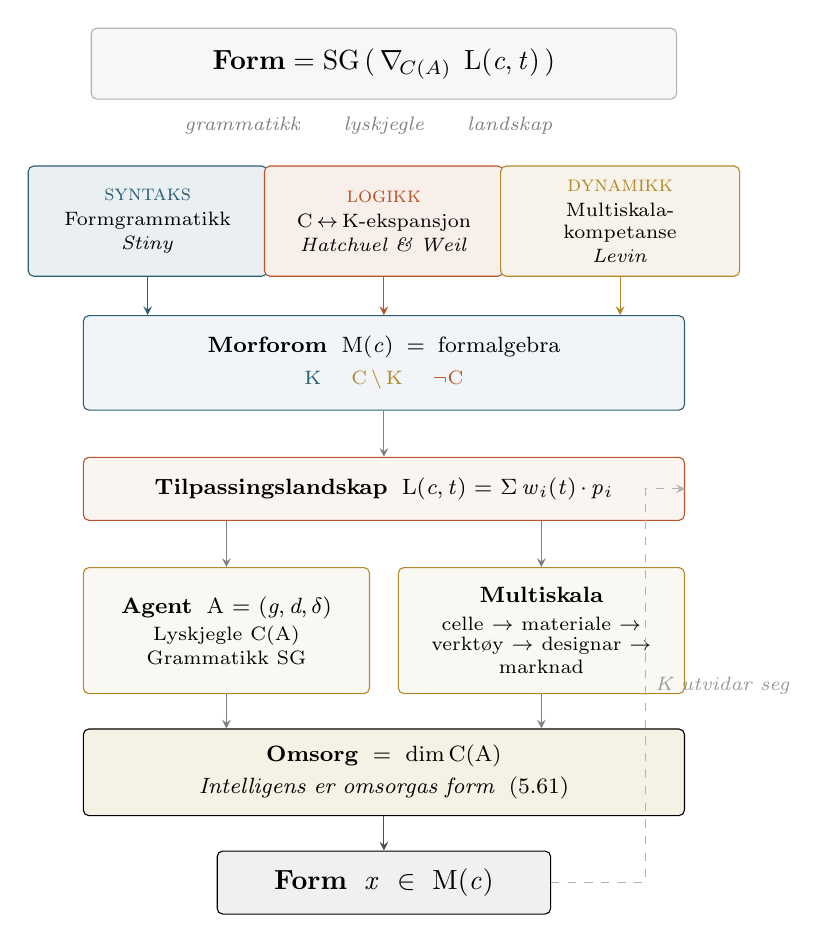
\begin{tikzpicture}[
  every node/.style={font=\footnotesize},
  box/.style={draw=#1, fill=#1!6, rounded corners=2pt,
              minimum height=8mm, text width=38mm, align=center,
              font=\footnotesize},
  pillar/.style={draw=#1, fill=#1!10, rounded corners=2pt,
                 minimum height=14mm, text width=28mm, align=center},
  arrow/.style={->, >=stealth, thin, #1},
  label/.style={font=\scriptsize\itshape, #1},
]

% ── Equation ──
\node[draw=black!30, fill=black!3, rounded corners=2pt,
      minimum height=9mm, text width=72mm, align=center]
  (eq) at (0, 8.2) {\normalsize\textbf{Form} = SG\,(\,$\nabla_{\!C(A)}$\, L(\textit{c},\,\textit{t})\,)};
\node[label=black!50, anchor=north] at (-1.8, 7.65) {grammatikk};
\node[label=black!50, anchor=north] at (0, 7.65) {lyskjegle};
\node[label=black!50, anchor=north] at (1.6, 7.65) {landskap};

% ── Three pillars ──
\definecolor{teal}{HTML}{2B5F75}
\definecolor{rust}{HTML}{B8542A}
\definecolor{gold}{HTML}{B4892A}

\node[pillar=teal] (sg) at (-3, 6.2)
  {\textsc{\color{teal}syntaks}\\[1pt]\scriptsize Formgrammatikk\\[-1pt]\scriptsize\textit{Stiny}};
\node[pillar=rust] (ck) at (0, 6.2)
  {\textsc{\color{rust}logikk}\\[1pt]\scriptsize C\,$\leftrightarrow$\,K-ekspansjon\\[-1pt]\scriptsize\textit{Hatchuel \& Weil}};
\node[pillar=gold] (tame) at (3, 6.2)
  {\textsc{\color{gold}dynamikk}\\[1pt]\scriptsize Multiskala-kompetanse\\[-1pt]\scriptsize\textit{Levin}};

% ── Morphospace ──
\node[box=teal, text width=74mm, minimum height=12mm] (morph) at (0, 4.4)
  {\textbf{Morforom}\; M(\textit{c})\;\;=\;\;formalgebra\\[2pt]
   \scriptsize\color{teal} K \quad\color{gold} C\,$\setminus$\,K \quad\color{rust} $\neg$C};

% ── Landscape ──
\node[box=rust, text width=74mm] (land) at (0, 2.8)
  {\textbf{Tilpassingslandskap}\; L(\textit{c},\,\textit{t}) = $\Sigma$\,\textit{w}$_i$(\textit{t})\,$\cdot$\,\textit{p}$_i$};

% ── Agent + Grammar ──
\node[box=gold, text width=34mm, minimum height=16mm] (agent) at (-2, 1.0)
  {\textbf{Agent}\; A = (\textit{g},\,\textit{d},\,\textit{$\delta$})\\[2pt]
   \scriptsize Lyskjegle C(A)\\[-1pt]
   \scriptsize Grammatikk SG};

% ── Multi-scale ──
\node[box=gold, text width=34mm, minimum height=16mm] (multi) at (2, 1.0)
  {\textbf{Multiskala}\\[2pt]
   \scriptsize celle $\to$ materiale $\to$\\[-1pt]
   \scriptsize verkt\o y $\to$ designar $\to$\\[-1pt]
   \scriptsize marknad};

% ── Care ──
\node[draw=black, fill=gold!12, rounded corners=2pt,
      minimum height=11mm, text width=74mm, align=center]
  (care) at (0, -0.8)
  {\textbf{Omsorg}\; =\; dim\,C(A)\\[2pt]
   \textit{Intelligens er omsorgas form}\;\;(5.61)};

% ── Form output ──
\node[draw=black, fill=black!6, rounded corners=2pt,
      minimum height=8mm, text width=40mm, align=center,
      font=\normalsize]
  (form) at (0, -2.2) {\textbf{Form}\; \textit{x}\; $\in$\; M(\textit{c})};

% ── Arrows ──
\draw[arrow=teal] (sg.south) -- (morph.north -| sg.south);
\draw[arrow=rust] (ck.south) -- (morph.north);
\draw[arrow=gold] (tame.south) -- (morph.north -| tame.south);

\draw[arrow=black!50] (morph.south) -- (land.north);
\draw[arrow=black!50] (land.south -| agent.north) -- (agent.north);
\draw[arrow=black!50] (land.south -| multi.north) -- (multi.north);

\draw[arrow=black!50] (agent.south) -- (care.north -| agent.south);
\draw[arrow=black!50] (multi.south) -- (care.north -| multi.south);
\draw[arrow=black!70] (care.south) -- (form.north);

% ── Feedback loop ──
\draw[arrow=black!30, dashed] (form.east) -- ++(1.2,0) |-
  node[pos=0.25, right, label=black!40] {K utvidar seg} (land.east);

\end{tikzpicture}
\end{figure}
 or compile standalone
\begin{figure}[p]
\centering
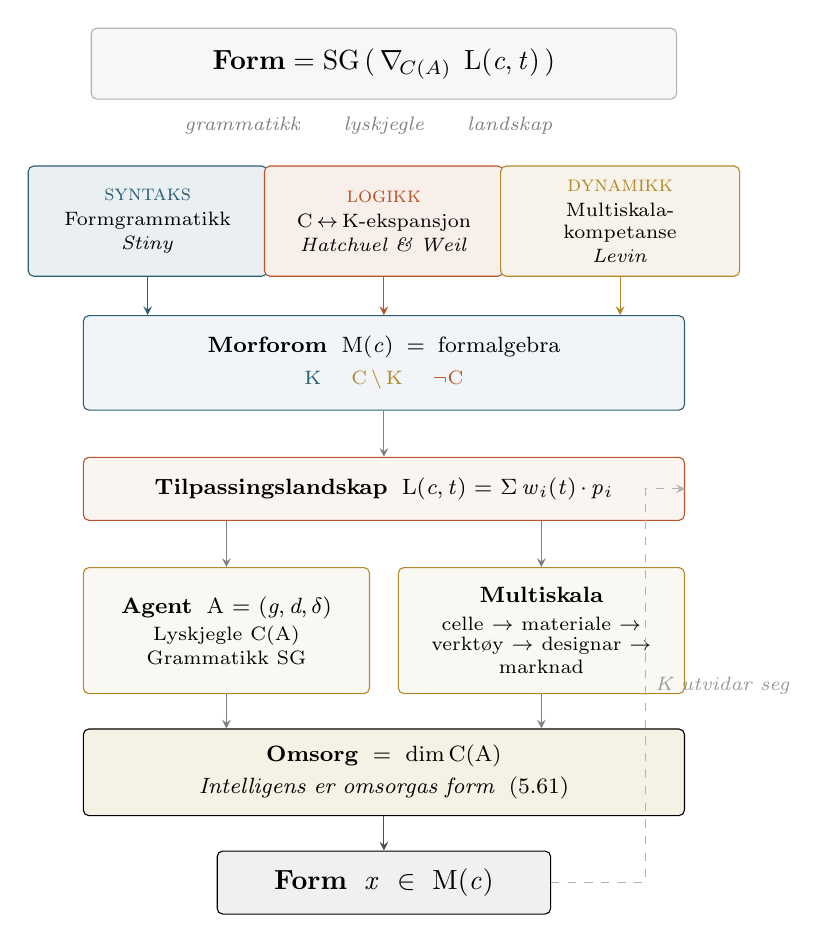
\begin{tikzpicture}[
  every node/.style={font=\footnotesize},
  box/.style={draw=#1, fill=#1!6, rounded corners=2pt,
              minimum height=8mm, text width=38mm, align=center,
              font=\footnotesize},
  pillar/.style={draw=#1, fill=#1!10, rounded corners=2pt,
                 minimum height=14mm, text width=28mm, align=center},
  arrow/.style={->, >=stealth, thin, #1},
  label/.style={font=\scriptsize\itshape, #1},
]

% ── Equation ──
\node[draw=black!30, fill=black!3, rounded corners=2pt,
      minimum height=9mm, text width=72mm, align=center]
  (eq) at (0, 8.2) {\normalsize\textbf{Form} = SG\,(\,$\nabla_{\!C(A)}$\, L(\textit{c},\,\textit{t})\,)};
\node[label=black!50, anchor=north] at (-1.8, 7.65) {grammatikk};
\node[label=black!50, anchor=north] at (0, 7.65) {lyskjegle};
\node[label=black!50, anchor=north] at (1.6, 7.65) {landskap};

% ── Three pillars ──
\definecolor{teal}{HTML}{2B5F75}
\definecolor{rust}{HTML}{B8542A}
\definecolor{gold}{HTML}{B4892A}

\node[pillar=teal] (sg) at (-3, 6.2)
  {\textsc{\color{teal}syntaks}\\[1pt]\scriptsize Formgrammatikk\\[-1pt]\scriptsize\textit{Stiny}};
\node[pillar=rust] (ck) at (0, 6.2)
  {\textsc{\color{rust}logikk}\\[1pt]\scriptsize C\,$\leftrightarrow$\,K-ekspansjon\\[-1pt]\scriptsize\textit{Hatchuel \& Weil}};
\node[pillar=gold] (tame) at (3, 6.2)
  {\textsc{\color{gold}dynamikk}\\[1pt]\scriptsize Multiskala-kompetanse\\[-1pt]\scriptsize\textit{Levin}};

% ── Morphospace ──
\node[box=teal, text width=74mm, minimum height=12mm] (morph) at (0, 4.4)
  {\textbf{Morforom}\; M(\textit{c})\;\;=\;\;formalgebra\\[2pt]
   \scriptsize\color{teal} K \quad\color{gold} C\,$\setminus$\,K \quad\color{rust} $\neg$C};

% ── Landscape ──
\node[box=rust, text width=74mm] (land) at (0, 2.8)
  {\textbf{Tilpassingslandskap}\; L(\textit{c},\,\textit{t}) = $\Sigma$\,\textit{w}$_i$(\textit{t})\,$\cdot$\,\textit{p}$_i$};

% ── Agent + Grammar ──
\node[box=gold, text width=34mm, minimum height=16mm] (agent) at (-2, 1.0)
  {\textbf{Agent}\; A = (\textit{g},\,\textit{d},\,\textit{$\delta$})\\[2pt]
   \scriptsize Lyskjegle C(A)\\[-1pt]
   \scriptsize Grammatikk SG};

% ── Multi-scale ──
\node[box=gold, text width=34mm, minimum height=16mm] (multi) at (2, 1.0)
  {\textbf{Multiskala}\\[2pt]
   \scriptsize celle $\to$ materiale $\to$\\[-1pt]
   \scriptsize verkt\o y $\to$ designar $\to$\\[-1pt]
   \scriptsize marknad};

% ── Care ──
\node[draw=black, fill=gold!12, rounded corners=2pt,
      minimum height=11mm, text width=74mm, align=center]
  (care) at (0, -0.8)
  {\textbf{Omsorg}\; =\; dim\,C(A)\\[2pt]
   \textit{Intelligens er omsorgas form}\;\;(5.61)};

% ── Form output ──
\node[draw=black, fill=black!6, rounded corners=2pt,
      minimum height=8mm, text width=40mm, align=center,
      font=\normalsize]
  (form) at (0, -2.2) {\textbf{Form}\; \textit{x}\; $\in$\; M(\textit{c})};

% ── Arrows ──
\draw[arrow=teal] (sg.south) -- (morph.north -| sg.south);
\draw[arrow=rust] (ck.south) -- (morph.north);
\draw[arrow=gold] (tame.south) -- (morph.north -| tame.south);

\draw[arrow=black!50] (morph.south) -- (land.north);
\draw[arrow=black!50] (land.south -| agent.north) -- (agent.north);
\draw[arrow=black!50] (land.south -| multi.north) -- (multi.north);

\draw[arrow=black!50] (agent.south) -- (care.north -| agent.south);
\draw[arrow=black!50] (multi.south) -- (care.north -| multi.south);
\draw[arrow=black!70] (care.south) -- (form.north);

% ── Feedback loop ──
\draw[arrow=black!30, dashed] (form.east) -- ++(1.2,0) |-
  node[pos=0.25, right, label=black!40] {K utvidar seg} (land.east);

\end{tikzpicture}
\end{figure}
 or compile standalone
\begin{figure}[p]
\centering
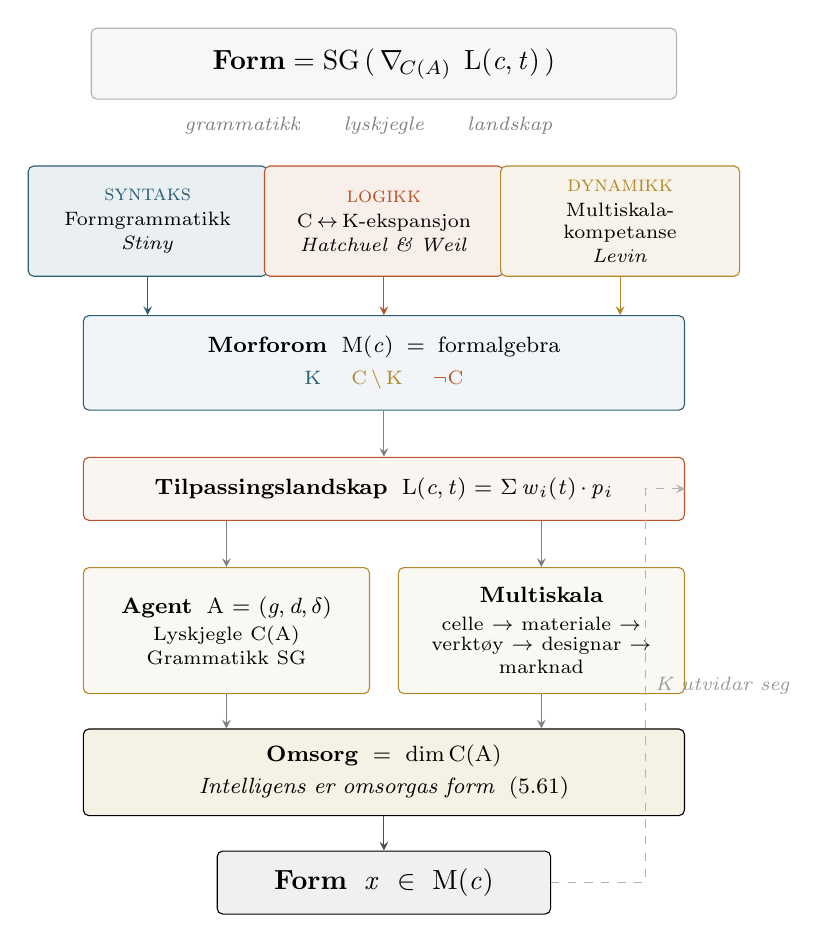
\begin{tikzpicture}[
  every node/.style={font=\footnotesize},
  box/.style={draw=#1, fill=#1!6, rounded corners=2pt,
              minimum height=8mm, text width=38mm, align=center,
              font=\footnotesize},
  pillar/.style={draw=#1, fill=#1!10, rounded corners=2pt,
                 minimum height=14mm, text width=28mm, align=center},
  arrow/.style={->, >=stealth, thin, #1},
  label/.style={font=\scriptsize\itshape, #1},
]

% ── Equation ──
\node[draw=black!30, fill=black!3, rounded corners=2pt,
      minimum height=9mm, text width=72mm, align=center]
  (eq) at (0, 8.2) {\normalsize\textbf{Form} = SG\,(\,$\nabla_{\!C(A)}$\, L(\textit{c},\,\textit{t})\,)};
\node[label=black!50, anchor=north] at (-1.8, 7.65) {grammatikk};
\node[label=black!50, anchor=north] at (0, 7.65) {lyskjegle};
\node[label=black!50, anchor=north] at (1.6, 7.65) {landskap};

% ── Three pillars ──
\definecolor{teal}{HTML}{2B5F75}
\definecolor{rust}{HTML}{B8542A}
\definecolor{gold}{HTML}{B4892A}

\node[pillar=teal] (sg) at (-3, 6.2)
  {\textsc{\color{teal}syntaks}\\[1pt]\scriptsize Formgrammatikk\\[-1pt]\scriptsize\textit{Stiny}};
\node[pillar=rust] (ck) at (0, 6.2)
  {\textsc{\color{rust}logikk}\\[1pt]\scriptsize C\,$\leftrightarrow$\,K-ekspansjon\\[-1pt]\scriptsize\textit{Hatchuel \& Weil}};
\node[pillar=gold] (tame) at (3, 6.2)
  {\textsc{\color{gold}dynamikk}\\[1pt]\scriptsize Multiskala-kompetanse\\[-1pt]\scriptsize\textit{Levin}};

% ── Morphospace ──
\node[box=teal, text width=74mm, minimum height=12mm] (morph) at (0, 4.4)
  {\textbf{Morforom}\; M(\textit{c})\;\;=\;\;formalgebra\\[2pt]
   \scriptsize\color{teal} K \quad\color{gold} C\,$\setminus$\,K \quad\color{rust} $\neg$C};

% ── Landscape ──
\node[box=rust, text width=74mm] (land) at (0, 2.8)
  {\textbf{Tilpassingslandskap}\; L(\textit{c},\,\textit{t}) = $\Sigma$\,\textit{w}$_i$(\textit{t})\,$\cdot$\,\textit{p}$_i$};

% ── Agent + Grammar ──
\node[box=gold, text width=34mm, minimum height=16mm] (agent) at (-2, 1.0)
  {\textbf{Agent}\; A = (\textit{g},\,\textit{d},\,\textit{$\delta$})\\[2pt]
   \scriptsize Lyskjegle C(A)\\[-1pt]
   \scriptsize Grammatikk SG};

% ── Multi-scale ──
\node[box=gold, text width=34mm, minimum height=16mm] (multi) at (2, 1.0)
  {\textbf{Multiskala}\\[2pt]
   \scriptsize celle $\to$ materiale $\to$\\[-1pt]
   \scriptsize verkt\o y $\to$ designar $\to$\\[-1pt]
   \scriptsize marknad};

% ── Care ──
\node[draw=black, fill=gold!12, rounded corners=2pt,
      minimum height=11mm, text width=74mm, align=center]
  (care) at (0, -0.8)
  {\textbf{Omsorg}\; =\; dim\,C(A)\\[2pt]
   \textit{Intelligens er omsorgas form}\;\;(5.61)};

% ── Form output ──
\node[draw=black, fill=black!6, rounded corners=2pt,
      minimum height=8mm, text width=40mm, align=center,
      font=\normalsize]
  (form) at (0, -2.2) {\textbf{Form}\; \textit{x}\; $\in$\; M(\textit{c})};

% ── Arrows ──
\draw[arrow=teal] (sg.south) -- (morph.north -| sg.south);
\draw[arrow=rust] (ck.south) -- (morph.north);
\draw[arrow=gold] (tame.south) -- (morph.north -| tame.south);

\draw[arrow=black!50] (morph.south) -- (land.north);
\draw[arrow=black!50] (land.south -| agent.north) -- (agent.north);
\draw[arrow=black!50] (land.south -| multi.north) -- (multi.north);

\draw[arrow=black!50] (agent.south) -- (care.north -| agent.south);
\draw[arrow=black!50] (multi.south) -- (care.north -| multi.south);
\draw[arrow=black!70] (care.south) -- (form.north);

% ── Feedback loop ──
\draw[arrow=black!30, dashed] (form.east) -- ++(1.2,0) |-
  node[pos=0.25, right, label=black!40] {K utvidar seg} (land.east);

\end{tikzpicture}
\end{figure}
 or compile standalone
\begin{figure}[p]
\centering
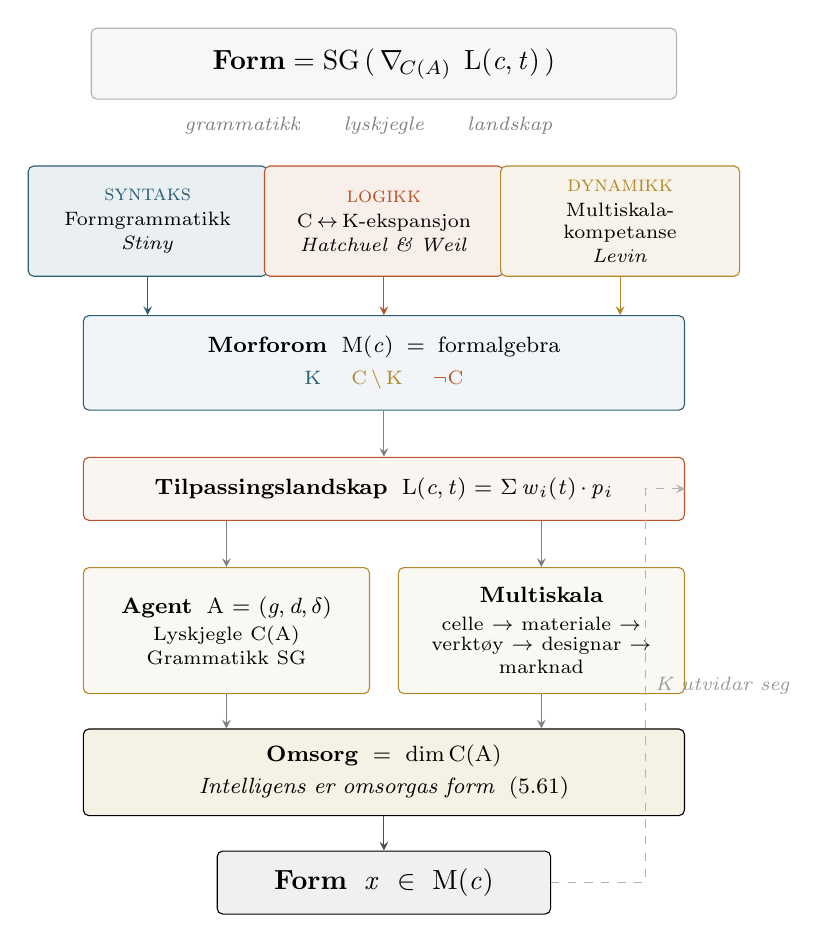
\begin{tikzpicture}[
  every node/.style={font=\footnotesize},
  box/.style={draw=#1, fill=#1!6, rounded corners=2pt,
              minimum height=8mm, text width=38mm, align=center,
              font=\footnotesize},
  pillar/.style={draw=#1, fill=#1!10, rounded corners=2pt,
                 minimum height=14mm, text width=28mm, align=center},
  arrow/.style={->, >=stealth, thin, #1},
  label/.style={font=\scriptsize\itshape, #1},
]

% ── Equation ──
\node[draw=black!30, fill=black!3, rounded corners=2pt,
      minimum height=9mm, text width=72mm, align=center]
  (eq) at (0, 8.2) {\normalsize\textbf{Form} = SG\,(\,$\nabla_{\!C(A)}$\, L(\textit{c},\,\textit{t})\,)};
\node[label=black!50, anchor=north] at (-1.8, 7.65) {grammatikk};
\node[label=black!50, anchor=north] at (0, 7.65) {lyskjegle};
\node[label=black!50, anchor=north] at (1.6, 7.65) {landskap};

% ── Three pillars ──
\definecolor{teal}{HTML}{2B5F75}
\definecolor{rust}{HTML}{B8542A}
\definecolor{gold}{HTML}{B4892A}

\node[pillar=teal] (sg) at (-3, 6.2)
  {\textsc{\color{teal}syntaks}\\[1pt]\scriptsize Formgrammatikk\\[-1pt]\scriptsize\textit{Stiny}};
\node[pillar=rust] (ck) at (0, 6.2)
  {\textsc{\color{rust}logikk}\\[1pt]\scriptsize C\,$\leftrightarrow$\,K-ekspansjon\\[-1pt]\scriptsize\textit{Hatchuel \& Weil}};
\node[pillar=gold] (tame) at (3, 6.2)
  {\textsc{\color{gold}dynamikk}\\[1pt]\scriptsize Multiskala-kompetanse\\[-1pt]\scriptsize\textit{Levin}};

% ── Morphospace ──
\node[box=teal, text width=74mm, minimum height=12mm] (morph) at (0, 4.4)
  {\textbf{Morforom}\; M(\textit{c})\;\;=\;\;formalgebra\\[2pt]
   \scriptsize\color{teal} K \quad\color{gold} C\,$\setminus$\,K \quad\color{rust} $\neg$C};

% ── Landscape ──
\node[box=rust, text width=74mm] (land) at (0, 2.8)
  {\textbf{Tilpassingslandskap}\; L(\textit{c},\,\textit{t}) = $\Sigma$\,\textit{w}$_i$(\textit{t})\,$\cdot$\,\textit{p}$_i$};

% ── Agent + Grammar ──
\node[box=gold, text width=34mm, minimum height=16mm] (agent) at (-2, 1.0)
  {\textbf{Agent}\; A = (\textit{g},\,\textit{d},\,\textit{$\delta$})\\[2pt]
   \scriptsize Lyskjegle C(A)\\[-1pt]
   \scriptsize Grammatikk SG};

% ── Multi-scale ──
\node[box=gold, text width=34mm, minimum height=16mm] (multi) at (2, 1.0)
  {\textbf{Multiskala}\\[2pt]
   \scriptsize celle $\to$ materiale $\to$\\[-1pt]
   \scriptsize verkt\o y $\to$ designar $\to$\\[-1pt]
   \scriptsize marknad};

% ── Care ──
\node[draw=black, fill=gold!12, rounded corners=2pt,
      minimum height=11mm, text width=74mm, align=center]
  (care) at (0, -0.8)
  {\textbf{Omsorg}\; =\; dim\,C(A)\\[2pt]
   \textit{Intelligens er omsorgas form}\;\;(5.61)};

% ── Form output ──
\node[draw=black, fill=black!6, rounded corners=2pt,
      minimum height=8mm, text width=40mm, align=center,
      font=\normalsize]
  (form) at (0, -2.2) {\textbf{Form}\; \textit{x}\; $\in$\; M(\textit{c})};

% ── Arrows ──
\draw[arrow=teal] (sg.south) -- (morph.north -| sg.south);
\draw[arrow=rust] (ck.south) -- (morph.north);
\draw[arrow=gold] (tame.south) -- (morph.north -| tame.south);

\draw[arrow=black!50] (morph.south) -- (land.north);
\draw[arrow=black!50] (land.south -| agent.north) -- (agent.north);
\draw[arrow=black!50] (land.south -| multi.north) -- (multi.north);

\draw[arrow=black!50] (agent.south) -- (care.north -| agent.south);
\draw[arrow=black!50] (multi.south) -- (care.north -| multi.south);
\draw[arrow=black!70] (care.south) -- (form.north);

% ── Feedback loop ──
\draw[arrow=black!30, dashed] (form.east) -- ++(1.2,0) |-
  node[pos=0.25, right, label=black!40] {K utvidar seg} (land.east);

\end{tikzpicture}
\end{figure}
